\section{Introducción}

        La espectroscopia de impedancia es una técnica de análisis de sistemas sensibles a señales eléctricas. Este se basa en la perturbación del objeto de estudio a través de una señal sinusoidal a lo largo de un rango de frecuencias adecuado, para luego analizar la respuesta del mismo en términos de la impedancia, una magnitud que relaciona la tensión aplicada con la corriente de un sistema \cite{Faulkner,Tutorial}. Entre sus principales ventajas con respecto a otros métodos de caracterización, existen tres propiedades que se destacan. En primer lugar, no requiere el desensamblaje del sistema, ya que solo son necesarias señales de entrada y salida. En segundo lugar, las medidas pueden ser realizadas en condiciones de operación normal, por lo que no se verán afectados los procesos llevados a cabo durante el experimento. Finalmente, la espectroscopia de impedancia es una técnica rápida y de bajo costo \cite{modeling}. Estas características favorecen su aplicación en una amplia variedad de sistemas electroquímicos, siendo el ejemplo más destacado el de las baterías de ion-litio.

        Las baterías de ion-litio son sistemas electroquímicos que convierten energía química en energía eléctrica a través de reacciones redox. Una caracterización posible para estos arreglos, es el de su \textit{estado de vida}, siendo este una medida de su degradación con respecto a cuando fue fabricada. Para poder realizar este análisis, es necesario conocer el comportamiento eléctrico de la batería, y debido a que este tiende a ser complejo, se lo modela con circuitos equivalentes que facilitan el estudio. En estos modelos, cada uno de los procesos físicos y electroquímicos que tienen lugar en la batería se representan mediante un elemento eléctrico. Las pérdidas óhmicas asociadas al electrolito, los electrodos y los contactos se modelan mediante resistencias, mientras que la acumulación de cargas en la interfaz electrodo-electrolito se representa mediante capacitores. Por otra parte, los procesos de difusión de iones en el electrolito y en los electrodos no pueden ser modelados mediante elementos eléctricos simples, por lo que se requiere la introducción de lo que se llama elemento de Warburg, concepto introducido por el físico alemán Emil Warburg en 1899 \cite{warburg}, particularmente para describir fenómenos difusivos en sistemas electroquímicos. Una vez obtenido el modelo de circuito equivalente, el \textit{estado de vida} de la batería puede ser determinado a partir de la desviación del valor de la resistencia total obtenida con respecto al valor presentado al momento de su ensamblaje \cite{modeling}.

\section{Marco teórico}
        Al aplicar una señal sinusoidal a un circuito, se puede definir la impedancia como la relación entre la tensión de entrada y la corriente a través del mismo. Como la corriente y la tensión son magnitudes sinusoidales desfasadas entre sí, la impedancia se puede expresar como una variable compleja, lo que lleva a que sea representada de la forma
        \begin{equation}
            Z(\omega) = \frac{V(\omega)}{I(\omega)} = |Z(\omega)|e^{i\phi(\omega)}
            \label{impedancia-general}
            \end{equation}
        A partir de la ecuación \eqref{impedancia-general}, se puede ver que existen dos formas de analizar el espectro frecuencial de la impedancia. La primera es a través de un diagrama de Bode, en el que se grafican la magnitud y la fase de la impedancia en función de la frecuencia en escala logarítmica, esto permite observar intervalos donde el circuito se vuelve inestable, por lo que resulta útil a la hora de estudiar sensores o filtros. La segunda es a través de un diagrama de Nyquist, en el que se grafican las partes real e imaginaria de la impedancia, lo que permite obtener un mejor conocimiento de los procesos que ocurren dentro del arreglo. Por ende, resulta útil a la hora de estudiar sistemas electroquímicos, donde lo que se busca es conocer la composición interna del sistema \cite{modeling}.

        En el caso de los circuitos eléctricos, la impedancia de cada uno de los elementos que lo componen se puede calcular a partir de las leyes de Kirchhoff y Ohm. Para una resistencia \(R\), la impedancia es simplemente \(Z_R = R\), mientras que para un capacitor \(C\), la impedancia es \(Z_C(\omega) = \frac{1}{i\omega C}\). En la \autoref{circuitos-ejemplo} se pueden observar ejemplos de diferentes circuitos RC junto a sus respectivos diagramas de Nyquist y Bode.

        \begin{figure}[H]
            \centering
            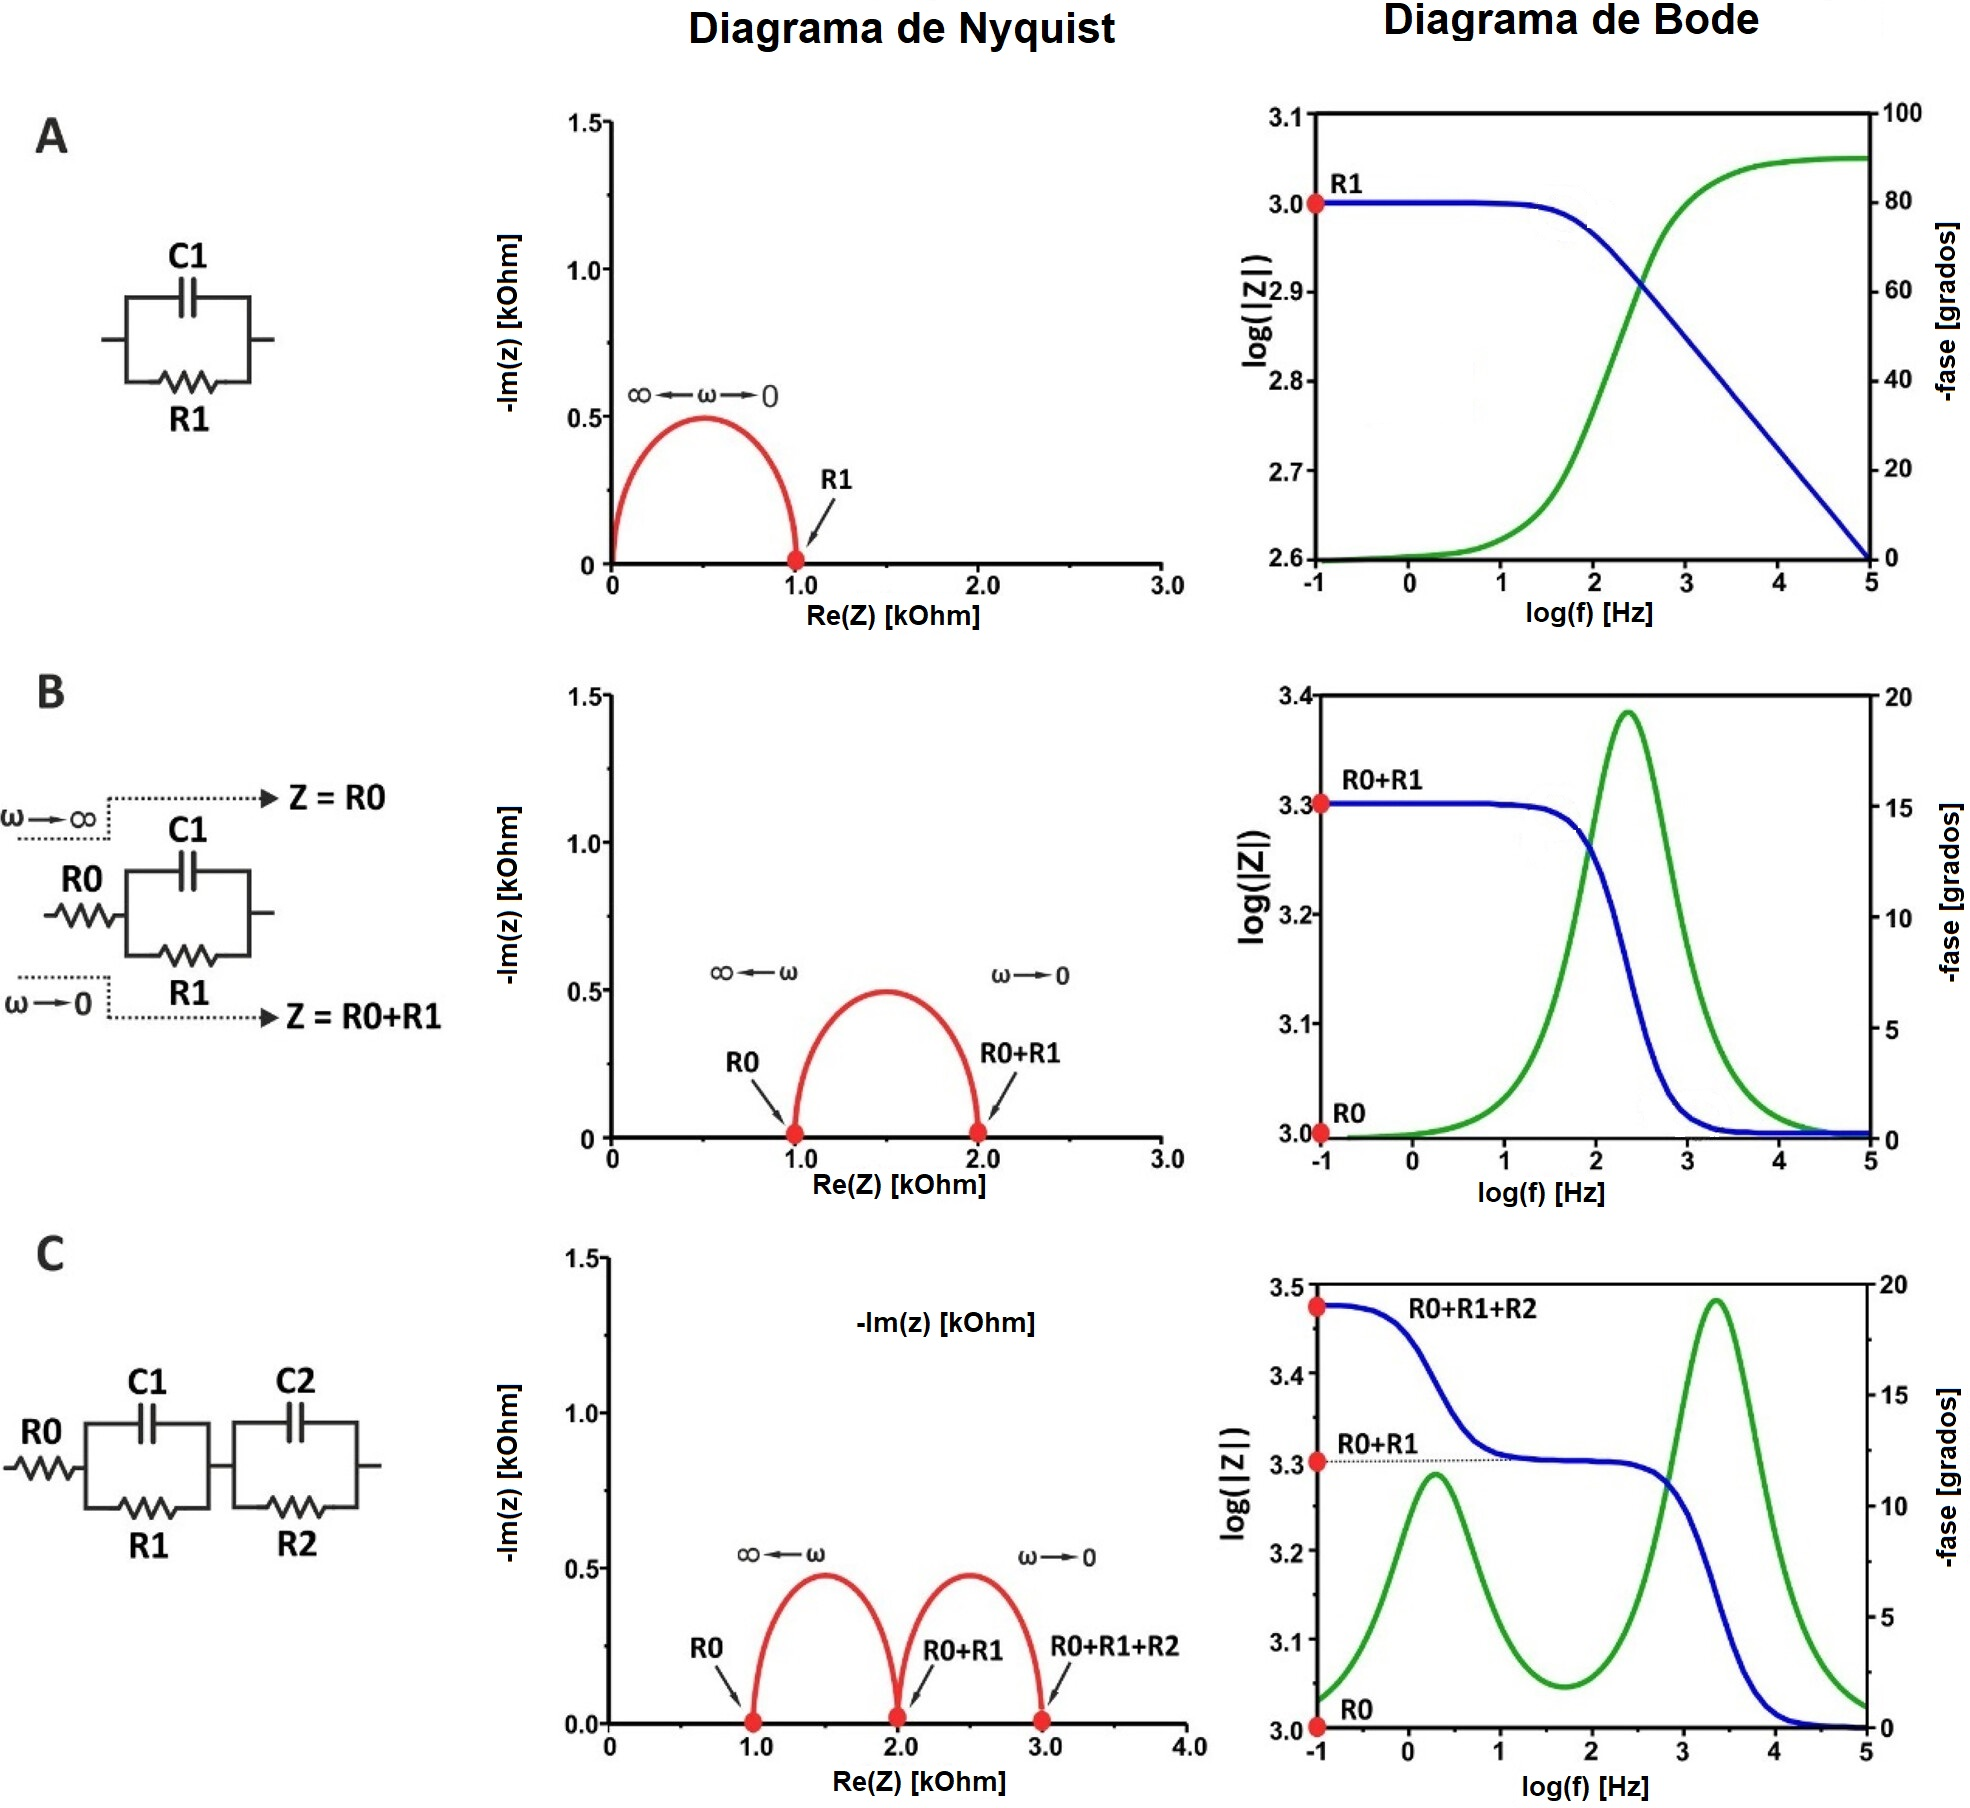
\includegraphics[width=0.5\textwidth]{Figuras/Circuitos_ejemplos.jpeg}
            \caption{Circuitos RC en serie, paralelo, y combinación de estos. En los tres casos \(C_i\) representan capacitores y \(R_i\) representan resistencias. Junto a ellos se muestran sus respectivos diagramas de Nyquist y Bode. Para los diagramas de Bode, la magnitud de la impedancia se representa en azul, mientras que la fase se representa en verde. En el caso de los diagramas de Nyquist, se muestran las respectivas curvas en rojo.}
            \label{circuitos-ejemplo}
        \end{figure}
        Por otro lado, como se mencionó anteriormente, es necesario introducir al elemento de Warburg para poder modelar determinados comportamientos en un circuito. Este componente es un caso particular de los elementos de fase constante (CPE, por sus siglas en inglés), los cuales son elementos cuya impedancia tiene un ángulo de fase constante en todo el rango de frecuencias. Su impedancia viene dada por
        \begin{equation}
            Z_{CPE}(\omega) = \frac{1}{Q(i\omega)^n}
            \label{CPE}
        \end{equation}
        donde \(Q\) es un parámetro cuyas unidades dependen de \(n\). Los valores de \(n\) varían de 0 a 1, siendo \(n=1\) y \(n=0\) los casos límites del CPE, donde se comporta como un capacitor y una resistencia respectivamente. El caso \(n=0.5\) corresponde a un elemento de Warburg \cite{cpe}.

        En este informe se estudiará el comportamiento de un circuito eléctrico del cual no se conoce su composición. Se realizarán mediciones de tensión de entrada y salida, las cuales se analizarán a través de la espectroscopia de impedancia. A partir de los resultados obtenidos, se buscará determinar el modelo del circuito equivalente que mejor represente al sistema.